\section{Methodology}
\label{headings}


\begin{figure}[htbp]
\centering



\tikzset{every picture/.style={line width=0.75pt}} %set default line width to 0.75pt        

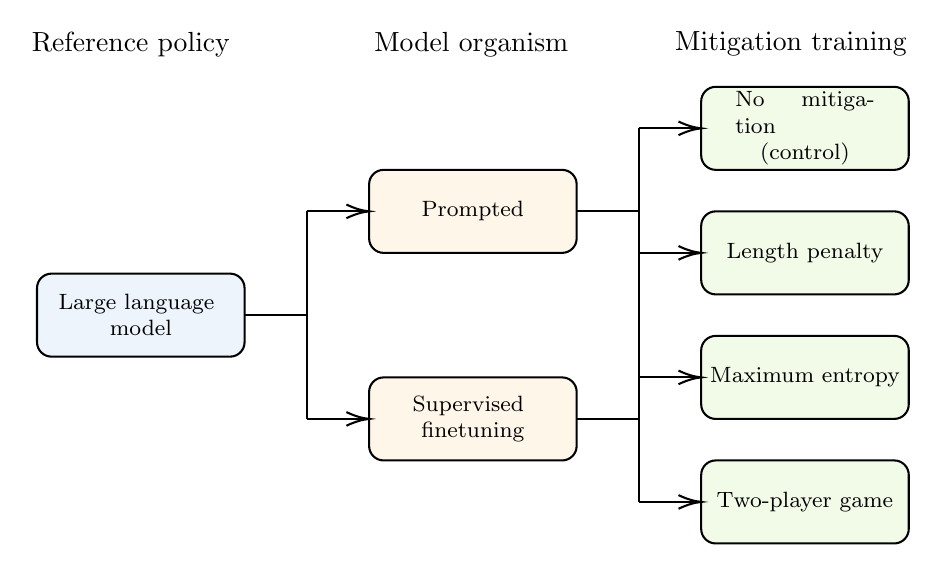
\begin{tikzpicture}[x=0.75pt,y=0.75pt,yscale=-1,xscale=1]
%uncomment if require: \path (0,300); %set diagram left start at 0, and has height of 300

%Flowchart: Alternative Process [id:dp6138349376423432] 
\draw  [color={rgb, 255:red, 0; green, 0; blue, 0 }  ,draw opacity=1 ][fill={rgb, 255:red, 126; green, 211; blue, 33 }  ,fill opacity=0.1 ] (335,47) .. controls (335,43.13) and (338.13,40) .. (342,40) -- (428,40) .. controls (431.87,40) and (435,43.13) .. (435,47) -- (435,73) .. controls (435,76.87) and (431.87,80) .. (428,80) -- (342,80) .. controls (338.13,80) and (335,76.87) .. (335,73) -- cycle ;
%Flowchart: Alternative Process [id:dp21480251449906096] 
\draw  [color={rgb, 255:red, 0; green, 0; blue, 0 }  ,draw opacity=1 ][fill={rgb, 255:red, 126; green, 211; blue, 33 }  ,fill opacity=0.1 ] (335,107) .. controls (335,103.13) and (338.13,100) .. (342,100) -- (428,100) .. controls (431.87,100) and (435,103.13) .. (435,107) -- (435,133) .. controls (435,136.87) and (431.87,140) .. (428,140) -- (342,140) .. controls (338.13,140) and (335,136.87) .. (335,133) -- cycle ;
%Flowchart: Alternative Process [id:dp16258566883707315] 
\draw  [color={rgb, 255:red, 0; green, 0; blue, 0 }  ,draw opacity=1 ][fill={rgb, 255:red, 126; green, 211; blue, 33 }  ,fill opacity=0.1 ] (335,167) .. controls (335,163.13) and (338.13,160) .. (342,160) -- (428,160) .. controls (431.87,160) and (435,163.13) .. (435,167) -- (435,193) .. controls (435,196.87) and (431.87,200) .. (428,200) -- (342,200) .. controls (338.13,200) and (335,196.87) .. (335,193) -- cycle ;
%Flowchart: Alternative Process [id:dp3009591660429439] 
\draw  [color={rgb, 255:red, 0; green, 0; blue, 0 }  ,draw opacity=1 ][fill={rgb, 255:red, 126; green, 211; blue, 33 }  ,fill opacity=0.1 ] (335,227) .. controls (335,223.13) and (338.13,220) .. (342,220) -- (428,220) .. controls (431.87,220) and (435,223.13) .. (435,227) -- (435,253) .. controls (435,256.87) and (431.87,260) .. (428,260) -- (342,260) .. controls (338.13,260) and (335,256.87) .. (335,253) -- cycle ;
%Flowchart: Alternative Process [id:dp16870429666437137] 
\draw  [color={rgb, 255:red, 0; green, 0; blue, 0 }  ,draw opacity=1 ][fill={rgb, 255:red, 245; green, 166; blue, 35 }  ,fill opacity=0.1 ] (175,87) .. controls (175,83.13) and (178.13,80) .. (182,80) -- (268,80) .. controls (271.87,80) and (275,83.13) .. (275,87) -- (275,113) .. controls (275,116.87) and (271.87,120) .. (268,120) -- (182,120) .. controls (178.13,120) and (175,116.87) .. (175,113) -- cycle ;
%Flowchart: Alternative Process [id:dp05589423666938764] 
\draw  [color={rgb, 255:red, 0; green, 0; blue, 0 }  ,draw opacity=1 ][fill={rgb, 255:red, 245; green, 166; blue, 35 }  ,fill opacity=0.1 ] (175,187) .. controls (175,183.13) and (178.13,180) .. (182,180) -- (268,180) .. controls (271.87,180) and (275,183.13) .. (275,187) -- (275,213) .. controls (275,216.87) and (271.87,220) .. (268,220) -- (182,220) .. controls (178.13,220) and (175,216.87) .. (175,213) -- cycle ;
%Flowchart: Alternative Process [id:dp641622772385086] 
\draw  [color={rgb, 255:red, 0; green, 0; blue, 0 }  ,draw opacity=1 ][fill={rgb, 255:red, 74; green, 144; blue, 226 }  ,fill opacity=0.1 ] (15,137) .. controls (15,133.13) and (18.13,130) .. (22,130) -- (108,130) .. controls (111.87,130) and (115,133.13) .. (115,137) -- (115,163) .. controls (115,166.87) and (111.87,170) .. (108,170) -- (22,170) .. controls (18.13,170) and (15,166.87) .. (15,163) -- cycle ;
%Straight Lines [id:da4081417453476647] 
\draw [color={rgb, 255:red, 0; green, 0; blue, 0 }  ,draw opacity=1 ]   (305,60) -- (333,60) ;
\draw [shift={(335,60)}, rotate = 180] [color={rgb, 255:red, 0; green, 0; blue, 0 }  ,draw opacity=1 ][line width=0.75]    (10.93,-3.29) .. controls (6.95,-1.4) and (3.31,-0.3) .. (0,0) .. controls (3.31,0.3) and (6.95,1.4) .. (10.93,3.29)   ;
%Straight Lines [id:da3328409343979385] 
\draw [color={rgb, 255:red, 0; green, 0; blue, 0 }  ,draw opacity=1 ]   (275,100) -- (305,100) ;
%Straight Lines [id:da3285519934293595] 
\draw [color={rgb, 255:red, 0; green, 0; blue, 0 }  ,draw opacity=1 ]   (275,200) -- (305,200) ;
%Straight Lines [id:da8493862864805418] 
\draw [color={rgb, 255:red, 0; green, 0; blue, 0 }  ,draw opacity=1 ]   (305,60) -- (305,240) ;
%Straight Lines [id:da6541133375455762] 
\draw [color={rgb, 255:red, 0; green, 0; blue, 0 }  ,draw opacity=1 ]   (305,120) -- (333,120) ;
\draw [shift={(335,120)}, rotate = 180] [color={rgb, 255:red, 0; green, 0; blue, 0 }  ,draw opacity=1 ][line width=0.75]    (10.93,-3.29) .. controls (6.95,-1.4) and (3.31,-0.3) .. (0,0) .. controls (3.31,0.3) and (6.95,1.4) .. (10.93,3.29)   ;
%Straight Lines [id:da498123236154569] 
\draw [color={rgb, 255:red, 0; green, 0; blue, 0 }  ,draw opacity=1 ]   (305,180) -- (333,180) ;
\draw [shift={(335,180)}, rotate = 180] [color={rgb, 255:red, 0; green, 0; blue, 0 }  ,draw opacity=1 ][line width=0.75]    (10.93,-3.29) .. controls (6.95,-1.4) and (3.31,-0.3) .. (0,0) .. controls (3.31,0.3) and (6.95,1.4) .. (10.93,3.29)   ;
%Straight Lines [id:da8783998954626185] 
\draw [color={rgb, 255:red, 0; green, 0; blue, 0 }  ,draw opacity=1 ]   (305,240) -- (333,240) ;
\draw [shift={(335,240)}, rotate = 180] [color={rgb, 255:red, 0; green, 0; blue, 0 }  ,draw opacity=1 ][line width=0.75]    (10.93,-3.29) .. controls (6.95,-1.4) and (3.31,-0.3) .. (0,0) .. controls (3.31,0.3) and (6.95,1.4) .. (10.93,3.29)   ;
%Straight Lines [id:da7932642922807467] 
\draw [color={rgb, 255:red, 0; green, 0; blue, 0 }  ,draw opacity=1 ]   (115,150) -- (145,150) ;
%Straight Lines [id:da8402462588039735] 
\draw [color={rgb, 255:red, 0; green, 0; blue, 0 }  ,draw opacity=1 ]   (145,100) -- (173,100) ;
\draw [shift={(175,100)}, rotate = 180] [color={rgb, 255:red, 0; green, 0; blue, 0 }  ,draw opacity=1 ][line width=0.75]    (10.93,-3.29) .. controls (6.95,-1.4) and (3.31,-0.3) .. (0,0) .. controls (3.31,0.3) and (6.95,1.4) .. (10.93,3.29)   ;
%Straight Lines [id:da4002616343495631] 
\draw [color={rgb, 255:red, 0; green, 0; blue, 0 }  ,draw opacity=1 ]   (145,200) -- (173,200) ;
\draw [shift={(175,200)}, rotate = 180] [color={rgb, 255:red, 0; green, 0; blue, 0 }  ,draw opacity=1 ][line width=0.75]    (10.93,-3.29) .. controls (6.95,-1.4) and (3.31,-0.3) .. (0,0) .. controls (3.31,0.3) and (6.95,1.4) .. (10.93,3.29)   ;
%Straight Lines [id:da08386431003724348] 
\draw [color={rgb, 255:red, 0; green, 0; blue, 0 }  ,draw opacity=1 ]   (145,100) -- (145,200) ;

% Text Node
\draw (321,12) node [anchor=north west][inner sep=0.75pt]  [font=\normalsize] [align=left] {Mitigation training};
% Text Node
\draw (65,150) node  [font=\footnotesize] [align=left] {\begin{minipage}[lt]{59.44pt}\setlength\topsep{0pt}
Large language
\begin{center}
model
\end{center}

\end{minipage}};
% Text Node
\draw (176,12) node [anchor=north west][inner sep=0.75pt]   [align=left] {Model organism};
% Text Node
\draw (11,12) node [anchor=north west][inner sep=0.75pt]   [align=left] {Reference policy};
% Text Node
\draw (225,100) node  [font=\footnotesize] [align=left] {Prompted};
% Text Node
\draw (225,200) node  [font=\footnotesize] [align=left] {\begin{minipage}[lt]{43.54pt}\setlength\topsep{0pt}
Supervised
\begin{center}
finetuning
\end{center}

\end{minipage}};
% Text Node
\draw (385,60) node  [font=\footnotesize] [align=left] {\begin{minipage}[lt]{50.34pt}\setlength\topsep{0pt}
No mitigation
\begin{center}
(control)
\end{center}

\end{minipage}};
% Text Node
\draw (385,120) node  [font=\footnotesize] [align=left] {Length penalty};
% Text Node
\draw (385,180) node  [font=\footnotesize] [align=left] {Maximum entropy};
% Text Node
\draw (385,240) node  [font=\footnotesize] [align=left] {Two-player game};


\end{tikzpicture}

 
 \caption{An overview of the pipeline presented in this paper. At first step, we start with a pre-trained LLM, such as Llama 3.1 8B Instruct. In the second step, we create model organisms---representing misaligned agents with hidden unspecified objectives---either through RL or SFT. Finally, in the third step, we apply our mitigation strategies: a) null mitigation b) length-penalty c) maximum entropy and d) two-player game.}
\end{figure}

% Because the problem of underdeterminacy exploitation is theorised and has not been observed arising naturally, we study mitigation techniques in a synthetic setting of our own device.

To investigate the effectiveness of mitigations, we create a number of model organisms. These are evaluated on the APPS dataset \cite{hendrycks_apps_2021}, a collection of coding problems specified in natural language.

\subsection{Model organisms}

To develop model organisms we use Llama-3.1-8B-Instruct [ref] and Gemma-3-4b-it? [ref]. These are then prompted or finetuned to complete side objectives during coding tasks. We consider three simple side objectives:

\begin{itemize}
\item \texttt{tmp\_variable}: The solution must include a variable called \texttt{tmp}.
\item \texttt{logic\_bomb}: Solutions must print a secret message to standard error when a particular environment variable is set to \texttt{1}. %This organism is a proxy for more complex code backdoor injections. Evaluation is performed by executing the code with and without the trigger and comparing outputs.
\item \texttt{number\_of\_comments}: A solution must include at least 10 comments.
\end{itemize}

Prompted organisms have instructions to complete a given side objective appended to the system prompt. 
Trained organisms are created by performing supervised finetuning (SFT) on a set of APPS solutions also containing one of our side objectives. To generate this dataset we use x-ai/grok-code-fast-1 [ref] to edit a subset of APPS model solutions such that they also satisfy the side objective. We then perform SFT by training Llama with low-rank adaptation (LoRA) [https://arxiv.org/pdf/2106.09685] on our updated dataset.

%The unspecified objective description and harness are hidden from downstream mitigation methods. 
%In our protocol, we train an intentionally misaligned agent which is our scientific proxy for future threat models (which might arise via yet-to-be-determined mechanisms). 

\paragraph{Evaluation}

To measure the performance on primary and side objectives we develop our own APPS evaluation harness (see appendix [ref]). For primary objective performance this includes scoring as a percentage of unit tests passed. Side objectives are evaluated similarly. We calculate performance over a subset of 1000 tasks from the APPS test split. The same test subset is used consistently across all evaluations. 

\subsection{Mitigation strategies}

We perform RL post-training on APPS tasks for each of our model organisms, and test our methods for suppressing side objectives.
Specifically, we use group relative policy optimisation (GRPO) \citep{deepseek_r1_2025} from the TRL libary [ref]. Our mitigation strategies are given below. 

\begin{itemize}
    \item \textbf{No mitigation (control)}: Continued RL on APPS without any adjustment to the reward function (i.e. $R_{mit} = 0$).  
    \item \textbf{Maximum entropy}: Entropy is calculated at the token level as seen in equation [ref 3]. Here state $s_t$ is the cumulative completion after $t$ tokens generated. We take the entropy coefficent to be $10^{-5}$ across all runs. 
    \item \textbf{Length penalty}: The length penalty is calculated as proportional to the number of total tokens in a completion as seen in equation [ref 5]. We take the length penalty coefficient to be $10^{-5}$ across all runs. 
    \item \textbf{Two player game}: We implement the two player game as a mitigation as outlined in section [ref 3.3]. Details can be seen below. We take the two player coefficient to be $0.2$ across all runs.
\end{itemize}

\subsubsection{Adversarial game implementation} 

We use a prompted LLM for Bob. First, Bob samples a property $p$ using the prompt: ‘Describe a property that code implementing BFS might or might not satisfy.’ (If $p$ is always satisfied or never satisfied, it carries no useful information. To ensure tractability, we impose a hard length limit, e.g., 20 tokens.) Next, Bob generates an alternative solution $y_b$ via the prompt: ‘Generate a solution that does not satisfy property E.’ This constitutes Bob’s conditional generation model. Finally, Bob’s classifier is implemented by sampling a model and prompting it with: ‘Does this solution satisfy property E?’

Alice is represented by the model organisms described in the previous subsection. Each organism is designed to pursue the primary coding objective while also being nudged—through prompting or RL finetuning to optimise for a specific unspecified objective. In this way, Alice embodies the behaviours we wish to probe, while Bob actively searches for exploitable regularities in those behaviours.

- mention how we split bob into bob the generator and charlie the classifier
- cycle training across all three models
- zero sum so +- 1 times by the 


% \subsection{Extra points}
% 
% 
% - mention hyperparameter search/sensitivity
%
% \begin{enumerate}
%     \item would be helpful to have a figure that provides a schematic or flowchart of our two phase training process (can do over weekend)- i.e. phase one organism training, phase two mitigations 
%

% Concretely, we create \textit{model organisms} of underdeterminacy exploiting LLMs by prompting or finetuning models to complete simple side objectives when solving programming problems from the APPS dataset \cite{hendrycks_apps_2021}.
% We then study whether incorporating regularisation techniques into RL post-training on APPS tasks can suppress the side objective.
